% Şekil: üçüncü harmonikli akımda referans, oluşan akım ve oransal denetleyici çıkışı (temsilî).
% İlk tezin Şekil 3.14'ünün (gömülü Excel grafiği) serilerinden çözülen bağıntılarla yeniden çizim:
% i* = sin(t), i = 0,8 sin(t) + 0,4 sin(3t), u = Kp (i* - i) = 0,2 sin(t) - 0,4 sin(3t), Kp = 1 (K-37).
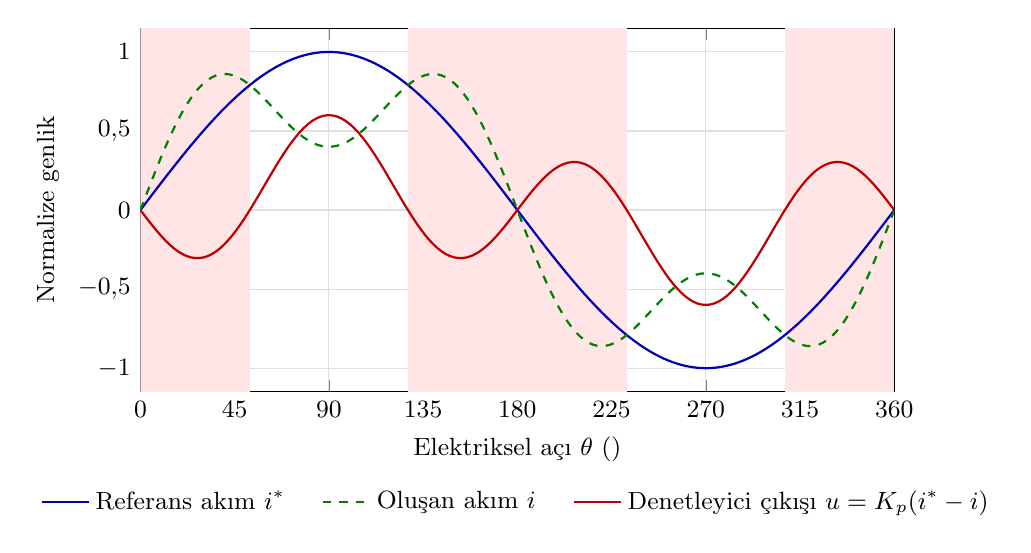
\begin{tikzpicture}
\begin{axis}[
  width=0.92\textwidth, height=62mm,
  tick label style={font=\fontsize{9}{10.5}\selectfont}, label style={font=\fontsize{9}{10.5}\selectfont},
  legend style={font=\fontsize{9}{10.5}\selectfont, at={(0.5,-0.24)}, anchor=north, legend columns=3, draw=none, /tikz/every even column/.append style={column sep=4mm}},
  xlabel={Elektriksel açı $\theta$ (\si{\degree})}, ylabel={Normalize genlik},
  xmin=0, xmax=360, ymin=-1.15, ymax=1.15,
  xtick={0,45,...,360}, ytick={-1,-0.5,0,0.5,1},
  /pgf/number format/use comma,
  grid=major, grid style={gray!25},
  domain=0:360, samples=181,
]
  % u'nun referansla ters isaretli oldugu araliklar: |sin t| < 0,79 (t = 52,2; 127,8; 232,2; 307,8 derece)
  \addplot[draw=none, fill=red!10, forget plot] coordinates {(0,-1.15) (52.24,-1.15) (52.24,1.15) (0,1.15)} -- cycle;
  \addplot[draw=none, fill=red!10, forget plot] coordinates {(127.76,-1.15) (232.24,-1.15) (232.24,1.15) (127.76,1.15)} -- cycle;
  \addplot[draw=none, fill=red!10, forget plot] coordinates {(307.76,-1.15) (360,-1.15) (360,1.15) (307.76,1.15)} -- cycle;
  \addplot[blue!70!black, thick] {sin(x)};
  \addlegendentry{Referans akım $i^{\ast}$}
  \addplot[green!50!black, thick, dashed] {0.8*sin(x)+0.4*sin(3*x)};
  \addlegendentry{Oluşan akım $i$}
  \addplot[red!75!black, thick] {0.2*sin(x)-0.4*sin(3*x)};
  \addlegendentry{Denetleyici çıkışı $u=K_p(i^{\ast}-i)$}
\end{axis}
\end{tikzpicture}
